\begin{figure}[ht]
\centering
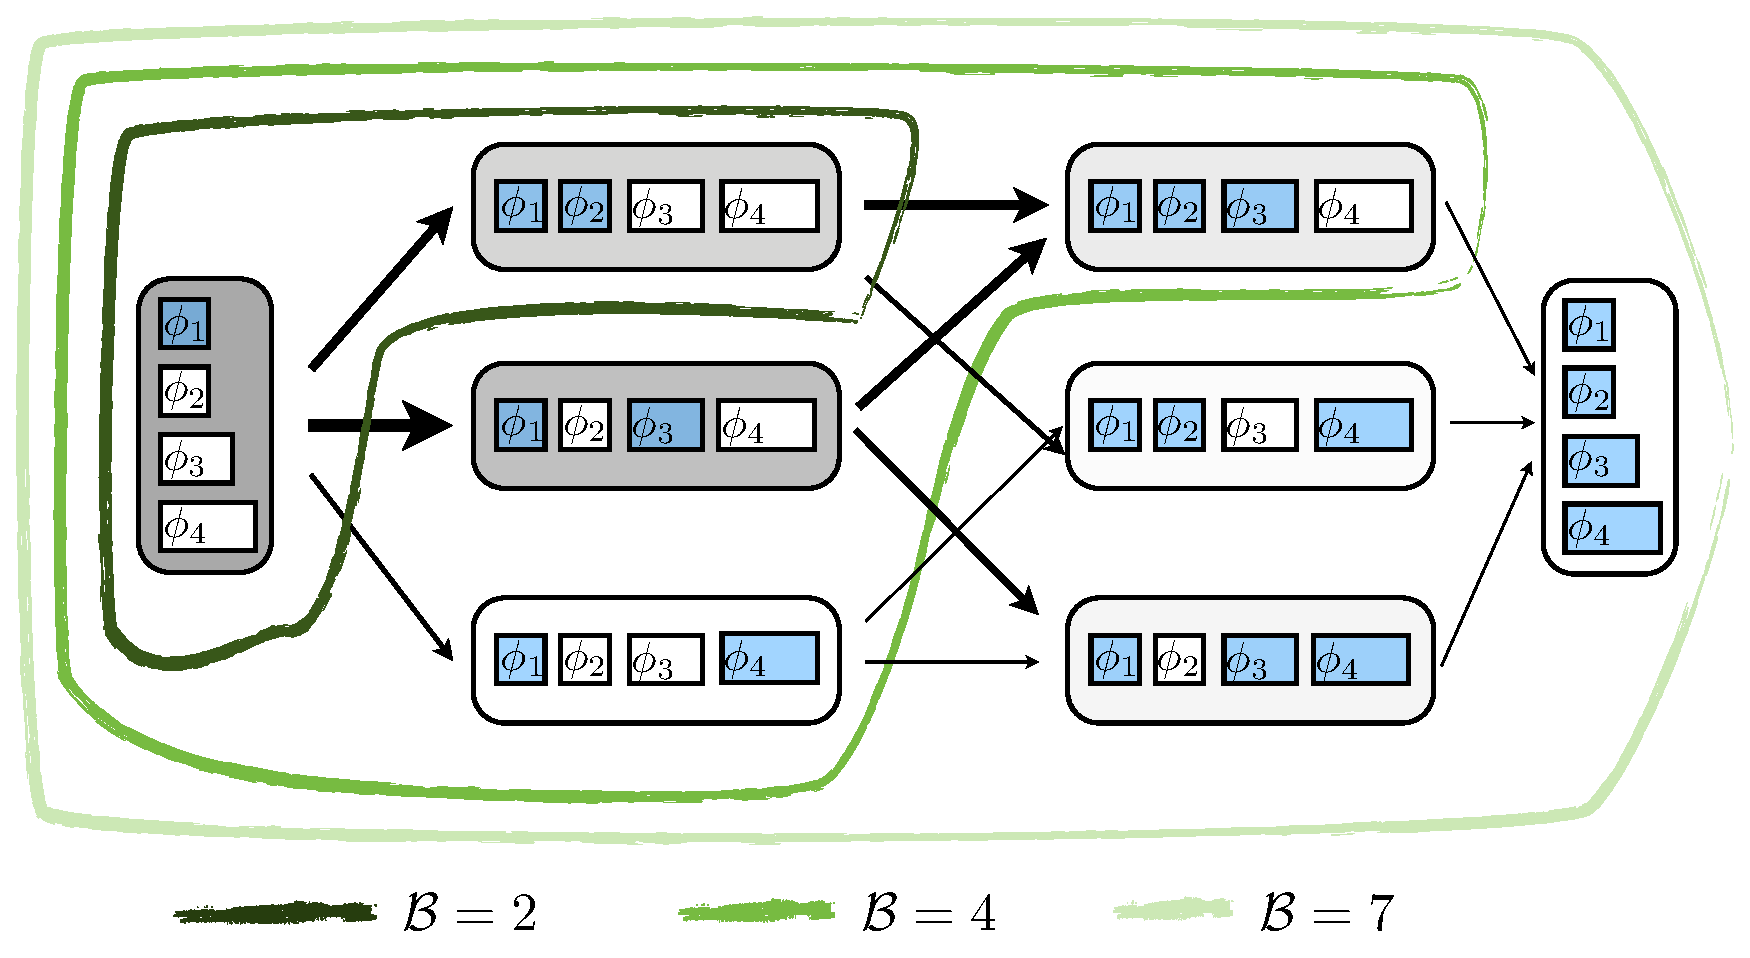
\includegraphics[width=.8\linewidth]{../../figures/mdp_masks.pdf}
\caption{
The action space $\mathcal{A}$ of the MDP is the the set of features $\mathcal{H}$, represented by the $\phi$ boxes.
The primary discretization of the state space can be visualized by the possible feature subsets (larger boxes); selected features are colored in the diagram.
The feature selection policy $\pi$ induces a distribution over feature subsets, for a dataset, which is represented by the shading of the larger boxes.
Not all states are reachable for a given budget $\mathcal{B}$.
In the figure, we show three ``budget cuts'' of the state space.
\label{fig:mdp_masks}
}
\end{figure}
